\vspace{-0.1cm}
\begin{figure}[tb]
    \centering
    \setlength{\belowcaptionskip}{-5pt}
    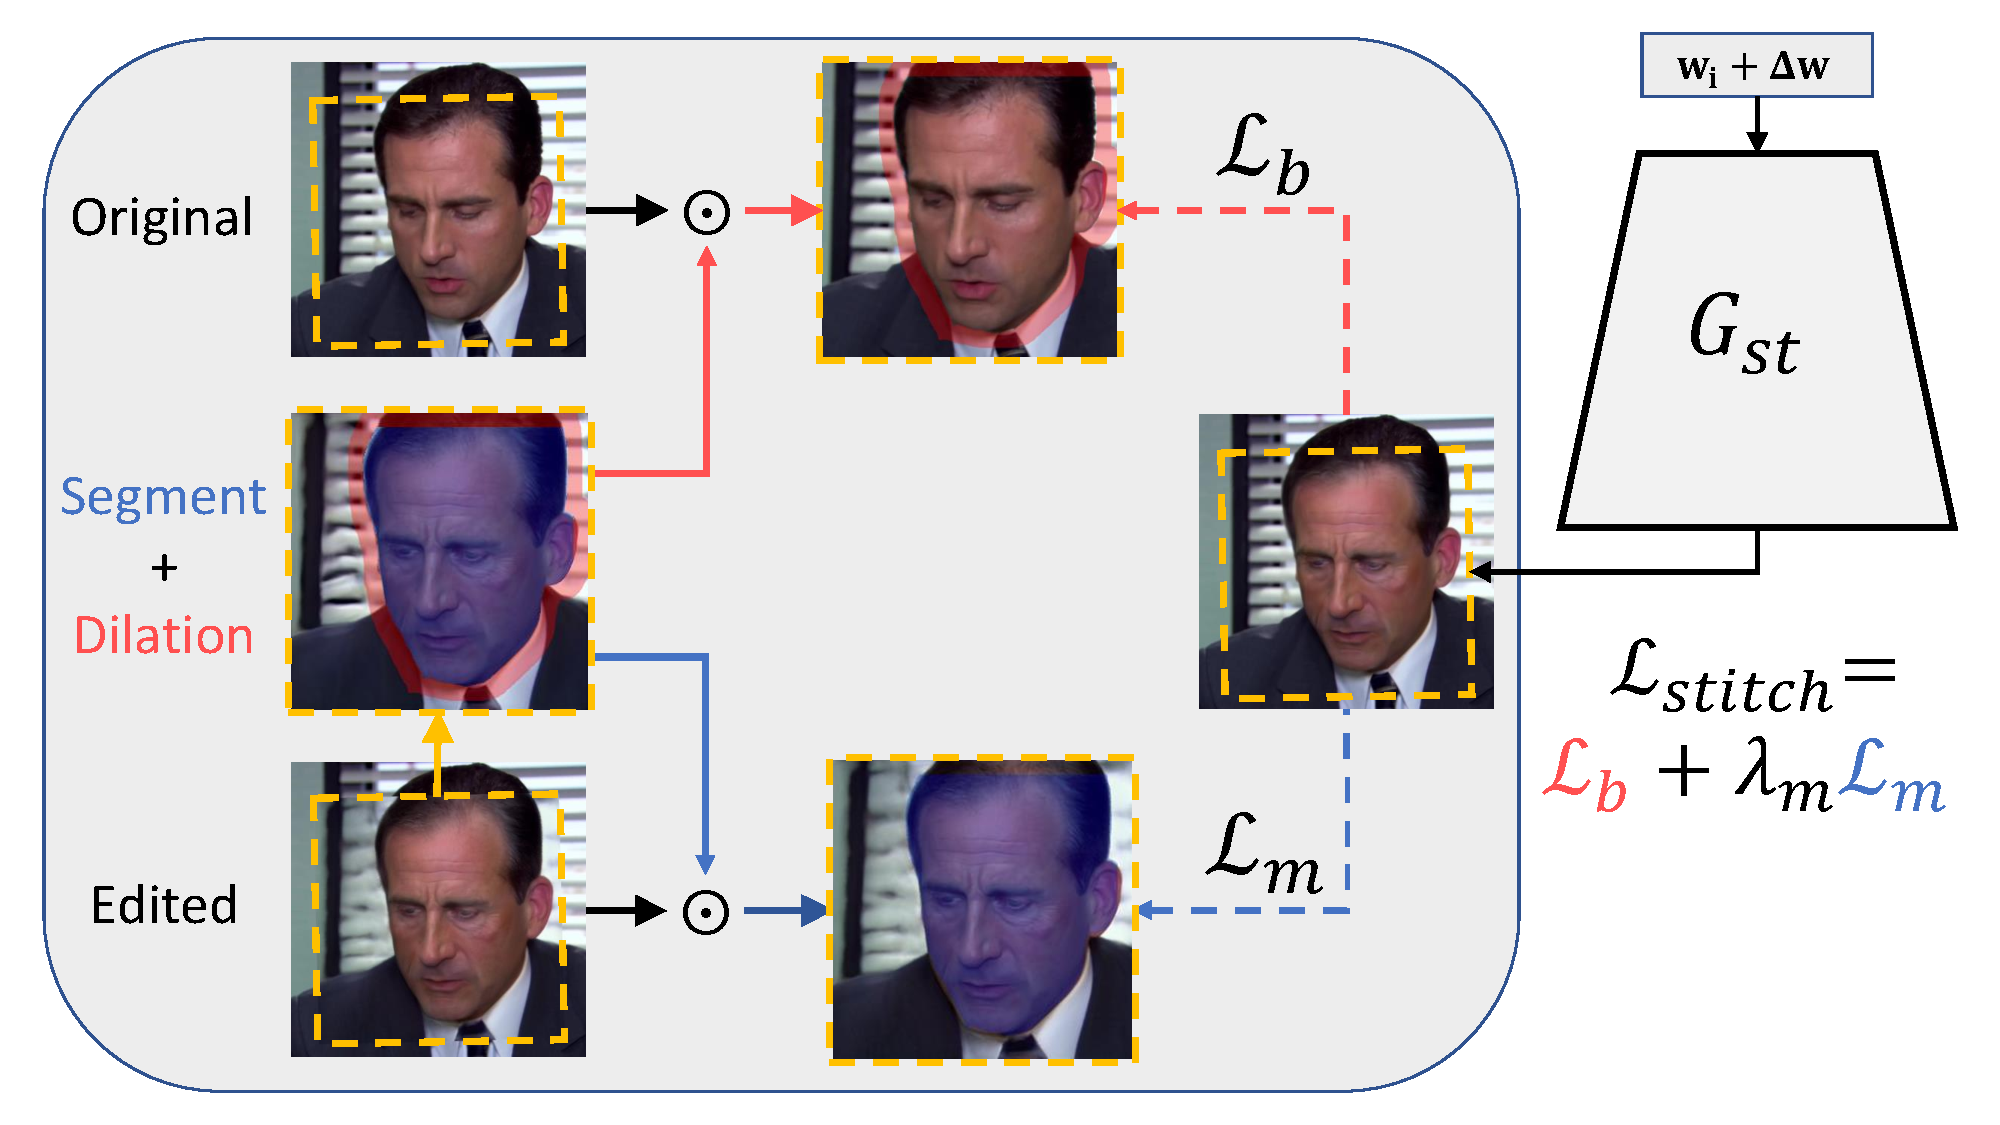
\includegraphics[width=0.99\linewidth]{resources/images/stitching.pdf}
    % \vspace{-0.25cm}
    \caption{
    Outline of our stitching-tuning method. We start with generating an edited image using a modified pivot code and segment the image using an off-the-shelf segmentation network \cite{yu2021bisenet}. The segmentation mask is dilated, creating a boundary region. We then fine-tune the generator so that the modified pivot will provide an image that is $(a)$ consistent with the original edit inside the face mask (blue), and $(b)$ consistent with the original background inside the boundary mask (red). We synthesize the final image using the tuned generator and paste it inside the dilated mask region (blue + red).
    }
    % \vspace{-0.2cm}
    \label{fig:stitching}
\end{figure}